\documentclass{scrartcl}

\usepackage{natbib}
\usepackage{hyperref}
\usepackage{amsmath}
\usepackage{verbatim}
\usepackage{listings}
\usepackage{color}
\usepackage{graphicx}


\usepackage{fvrb-ex}
\fvset{gobble=0,numbersep=3pt}
\fvset{numbers=left,frame=single}
%\RecustomVerbatimEnvironment{Verbatim}{Verbatim}{commandchars=§µ¶}
\DefineVerbatimEnvironment%
{CVerbatim}{Verbatim}
{fontfamily=tt,fontsize=\small,frame=single,formatcom=\color{blue},label=\emph{Interactive Stata example}}
\DefineVerbatimEnvironment{Sinput}{Verbatim}{fontshape=sl,formatcom=\color{blue}}


\lstset{ %
  basicstyle=\tiny\ttfamily\color{blue}, %
  frame=single, %
  includerangemarker = false, %
  title = \footnotesize\ttfamily\color{blue}\emph{Interactive Stata Example}, %
  captionpos = t, %
  rangeprefix=*@*, %
  %belowcaptionskip = -0.08in, %
  label={bla}
}

\lstnewenvironment{stata}
  {label=blabla}{}

\begin{document}

	\title{Homework assignment \#6\\ Panel Data Analysis}
	\subtitle{MPP-C6: Statistics 2}
	\author{Prof. Jan C. Minx\\ \texttt{minx@hertie-school.org} \\
		\url{http://moodle.hertie-school.org/course/view.php?id=1192}}
	\date{29 October 2015}
	
	\maketitle
	
	\indent\textbf{Disclaimer: This document sketches some brief responses to the questions of the homework assignment. It serves to provide students with some guidance. The document may include som flaws - those should be reported to me as students go through the responses.}

	\subsection*{Project Description}
	The Environmental Kuznets Curve is at the heart of a long-standing discourse on the relationship between economic development and environmental quality. It hypothesizes an inverted U-shape relationship between indicators of environmental degradation and per capita income. While some have used the EKC to argue that growth policies are also superior for dealing with environmental problems, others have questioned the existence of EKCs for different indicators or stressed very high turning points. We aim to reproduce the results of Stern and Common (2001) which sought to investigate the presence of an environmental Kuznets curve (EKC) for sulfur emissions \cite{stern2001there}.
	
	\subsection*{Dataset}
	The dataset stern2.dat contains country data from 1960-1990. The dataset contains the following variables
	\begin{itemize}
	\item \textit{year}: the year in which the country was observed 
	\item \textit{country}: numerical code that uniquely identifies each country (see table 1)
	\item \textit{gdpppp}: GDP per capita (purchasing power parity) in real 1990 international dollars
	\item \textit{pop}: population in 1000 residents
	\item \textit{so}: \(SO_2\) emissions in tonnes
	\item \textit{sopc}: \(SO_2\) emissions in tonnes per capita
	\item \textit{oe}: dummy variable describing oecd membership where 1000 represents membership and 2000 represents non-membership
	\end{itemize}
	
	\subsection*{Questions}
	
	\begin{enumerate}
	\item \textbf{Read the paper by Stern and Common. Explain the EKC hypothesis in your own words. What is the difference between sulfur and carbon emissions in the empirical discussion and why? What is the authors' perceived contribution to the discussion? What is the role of panel data therein? [conceptual question]}
	
	The EKC hypothesis estimates that an inverted U-shape describes the relationship between income per capita and measures of environmental degradation. In other words, at low levels of income, increases in income will be associated with increases in environmental degradation, but as income rises, the effect will become smaller until a turning point, beyond which increases in income per capita will lead to decreases in environmental degradation.
	
	It was thought that carbon had a high turning point and sulfur had a low turning point, because the externalities of carbon emissions are global, whereas the externalities of sulfur emissions are local.
	
	The authors believe that previous estimates of an EKC for sulfur underestimate the turning point by relying on a sample of higher income countries. Panel data helps to control for time and country effects.
		
	\item \textbf{Start by examining your data. Try out some descriptive statistics of the xt command family and report relevant ones. What sort of distribution do our variables of interest display? What transformations could we apply to the data? If necessary, create new variables that are appropriately transformed.}
	
	\lstinputlisting[linerange={lstart-lend}]{../stata/stern_assignment_q2.log}

	\begin{figure}
      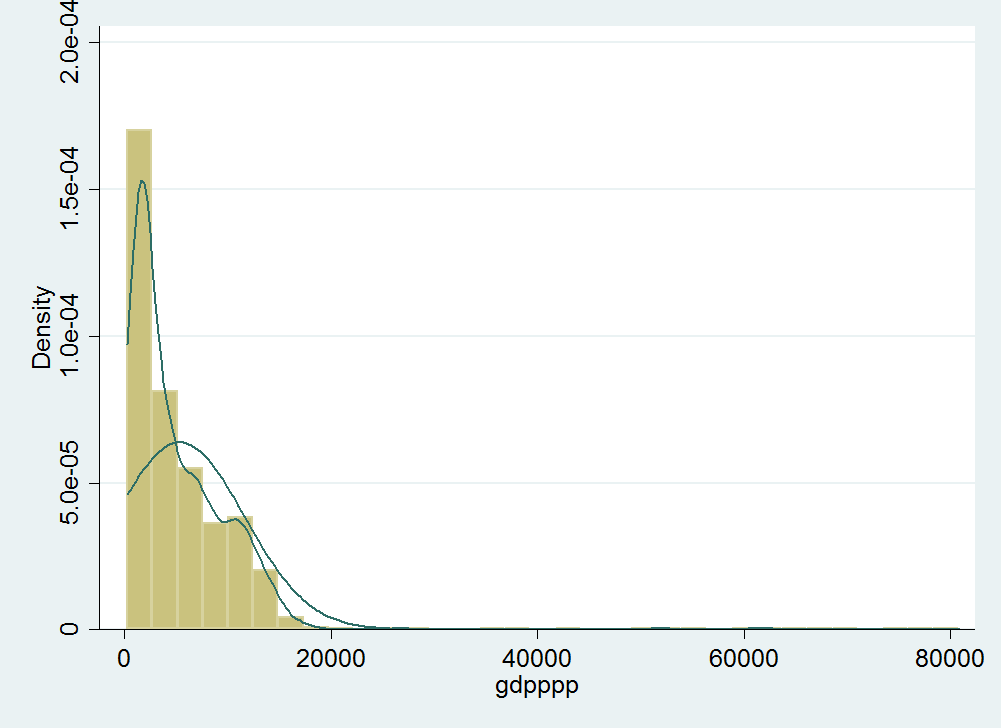
\includegraphics[width=10cm]{../stata/hist_gdp.png}
      \caption{GDP distribution}
    \end{figure}

	\begin{figure}
      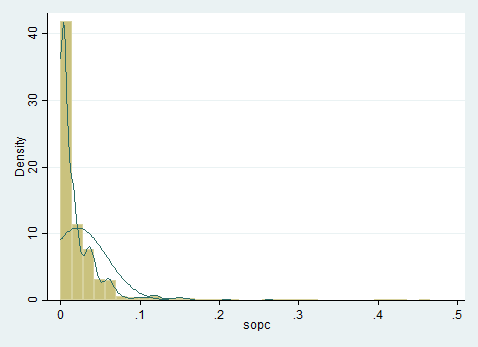
\includegraphics[width=10cm]{../stata/hist_sopc.png}
      \caption{Sopc distribution}
    \end{figure}

	Both variables are right-skewed (see figures 1 and 2), so a log transformation is appropriate.
	
	\item \textbf{Plot GDP per capita against sulfur emissions per capita (transformed if necessary). Describe the relationship you can see.}
	
	\lstinputlisting[linerange={lstart-lend}]{../stata/stern_assignment_q3.log}
	
	At low levels of income, a positive effect of GDP per capita on sulphur emissions per capita is clearly visible. There seems to be some sign of a turning point, but it is not unambiguous (see figure 3).
	
	 \begin{figure}
      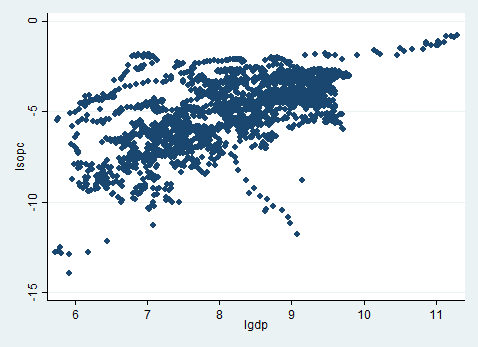
\includegraphics[width=12cm]{../stata/lsopc_lgdp.png}
      \caption{log GDP per capita against log sulfur emissions per capita}
    \end{figure}
	
	\item \textbf{Write the equation for a model that could estimate an EKC for sulfur emissions. Create any extra variables that would be necessary to run this.}
	
	\[ \ln{SO_i} = \beta_0 + \beta_1 lgdp + \beta_2 lgdp^2\]
	
	
	\item \textbf{Carry out a pooled regression using the equation described in question 3. Interpret the coefficients. Run fixed-effects and random-effects models and interpret the results.}

	\lstinputlisting[linerange={lstart-lend}]{../stata/stern_assignment_q5.log}
	
	A Pooled regression finds a positive, significant coefficient for the linear GDP term. The squared GDP term is negative but insignificant. We would estimate the turning point of the EKC as \[ \tau = \exp\left(\frac{-\beta_1}{2\cdot\beta_2}\right) = 2949748538 \] This is far outside our sample and an unreasonable value for GDP per capita.

	Both fixed effects models and random effects models find larger effects for both the linear term and the squared term, and the squared term is significant in each. In the case of the fixed effects model the turning point is estimated as 42736.09, the turning point in the random effects model is estimated as 46078.71.
	
	\item \textbf{Test which of the three models is preferable. Perform other relevant diagnostics for the model of choice. Is it appropriate to include time-fixed effects in the model?}
	
	\lstinputlisting[linerange={lstart-lend}]{../stata/stern_assignment_q6.log}
	
	A Breusch-Pagan test conducted on the pooled OLS model informs us that we should reject the null hypothesis that the model does not suffer from heteroskedasticity. This means that we should consider fixed effects and random effects models.
	
	A Hausman test compares the coefficients of the fixed and random effects models. It finds that the difference between them is significant. A significant difference indicates that the random effects model is esti-
mated inconsistently, due to correlation between the explanatory variables and the
error components.	We should therefore prefer a fixed-effects model.
	
	\item \textbf{What is heterogeneity bias and is it relevant according to your results? [conceptual question]}
	
	Heterogeneity bias comes from ignoring the individual or time-specific effects that exist among cross-sectional or time-series units but are not captured by the included explanatory variables. If the characteristics of individual countries in our dataset that are not captured by our explanatory variables have an effect on sulphur emissions, then a pooled OLS reression will be biased.
	
	\item \textbf{A high Hausman statistic implies that there is correlation between country effects and income variables. What could be the most likely cause of this problem? [conceptual question]}
	
	This could be caused by country attributes that both make countries richer and affect their sulphur emissions.
		
	\item \textbf{Compute the relevant turning points of the estimated curves for the world, OECD and non-OECD regressions. Summarize your results in a table.}
	
	\lstinputlisting[linerange={lstart-lend}]{../stata/stern_assignment_q9.log}
		
	\item \textbf{Discuss why first-differencing may be a more appropriate method for the data.}
	
	Differencing reduces the serial correlation and removes the country effects that are related to the specification problems in the levels model. If there are omitted integrated variables the first
differences estimator is consistent.
	
	\item \textbf{Estimate the model for the ``world'' using first-differences and interpret the results.}
	
	\lstinputlisting[linerange={lstart-lend}]{../stata/stern_assignment_q11.log}
	
	A first differencing model shows a smaller coefficient for both the linear and squared gdp terms, though both are significant. The turning point is estimated as 84276.43
	
	\item \textbf{Comment on any differences between the models you have run.}
	
	Pooled OLS found no significant turning point for an EKC for sulfur emissions. 
	
	Fixed and random effects models estimated similar turning points at around 43000 and 46000 respectively, though we preferred fixed-effects based on a high Hausman statistic. Further analysis showed that the fixed-effects estimate was highly dependent on the sample. Excluding or including OECD and non-OECD countries changed the turning point estimate significantly. 
	
	A first differencing model, which may be preferable, estimated a much higher turning point close to 84000. 
	
	\item \textbf{Discuss whether we can observe an EKC for sulfur emissions with reference to your results.}
	
	We can conclude that a single global EKC model is misspecified. The estimation of the turning point is heavily dependent on the countries in the sample. However, fixed-effects, random-effects and first-difference models all find a significant turning point for sulfur emissions, though for first-difference model the turning point is higher than the maximum GDP value in the sample.
	
	\end{enumerate}
	


	%\stata[linerange={8-26}]{../stata/stern_assignment_q5.log}
	
	\begin{table}[h!]\caption{Country Codes}\label{tab:imp}
	\begin{center}
	
\begin{tabular}{|l|c|l|c|}

\hline

1 & ALGERIA     &       95  &JAPAN       \\
14& EGYPT       &       97  &KOREA,      \\
18& GHANA       &       98  &KUWAIT      \\
22& KENYA       &       100 &MALAYSIA    \\
25& MADAGASCAR  &       102 &MYANMAR    \\
30& MOROCCO     &       106 &PHILIPPINES     \\
31& MOZAMBIQUE  &       108 &SAUDI ARABIA    \\
32& NAMIBIA     &       109 &SINGAPORE   \\
34& NIGERIA     &       110 &SRI LANKA   \\
41& SAFRICA     &       111 &SYRIA       \\
44& TANZANIA    &       112 &TAIWAN      \\
46& TUNISIA     &       113 &THAILAND    \\
48& ZAIRE       &       116 &AUSTRIA     \\
49& ZAMBIA      &       117 &BELGIUM    \\
50& ZIMBABWE    &       119 &CYPRUS      \\
52& BARBADOS    &       120 &CZECHOSLOVAKIA  \\
54& CANADA      &       121 &DENMARK     \\
60& GUATEMALA   &       122 &FINLAND    \\
62& HONDURAS    &       123 &FRANCE      \\
64& MEXICO      &       125 &WGERMANY    \\
65& NICARAGUA   &       126 &GREECE      \\
71& TRINIDAD\&TOBAGO&       129 &IRELAND    \\
72& U.S.A.      &       130 &ITALY       \\
73& ARGENTINA   &       131 &LUXEMBOURG  \\
74& BOLIVIA     &       133 &NETHERLANDS     \\
75& BRAZIL      &       134 &NORWAY      \\
76& CHILE       &       136 &PORTUGAL    \\
77& COLOMBIA    &       137 &ROMANIA    \\
81& PERU        &       138 &SPAIN       \\
83& URUGUAY     &       139 &SWEDEN      \\
84& VENEZUELA   &       140 &SWITZERLAND     \\
88& CHINA       &       141 &TURKEY      \\
89& HONG KONG   &       142 &U.K.        \\
90& INDIA       &       143 &USSR        \\
91& INDONESIA   &       144 &YUGOSLAVIA  \\
92& IRAN        &       145 &AUSTRALIA   \\
94& ISRAEL      &       147 &NZ      \\
\hline
\end{tabular}
\end{center}
\end{table}

\bibliography{lit_h6}
\bibliographystyle{plain}

\end{document}
